\subsubsection{UC12 - Effettua una prenotazione}
\begin{figure}[h]
	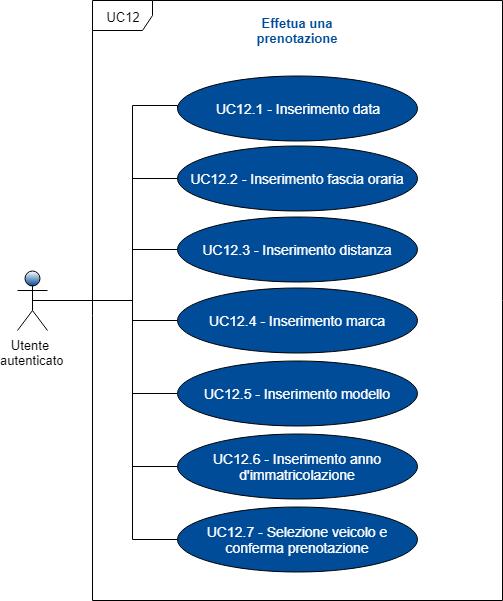
\includegraphics[width=10cm]{res/images/UC12Effettuaprenotazione.png}
	\centering
	\caption{UC12 - Effettua una prenotazione}
\end{figure}
\begin{itemize}
	\item \textbf{Attori Primari}: utente autenticato;
	\item \textbf{Descrizione}: l'utente può ricercare un veicolo sfruttando diversi parametri e prenotare quello più adatto alle sue esigenze.
	\item \textbf{Scenario principale}: l'utente per effettuare la prenotazione di un veicolo avrà a disposizione una maschera di ricerca che gli permetterà di filtrare i veicoli secondo questi parametri:
	\begin{itemize}
		\item data [UC12.1];
		\item fascia oraria [UC12.2];
		\item distanza: l'utente può inserire un raggio in chilometri per selezionare solo i veicoli presenti nell'area circoscritta [UC12.3]; 
		\item marca [UC12.4];
		\item modello [UC12.5];
		\item anno d'immatricolazione [UC12.6].
	\end{itemize}
	L'utente avrà quindi a disposizione una lista di veicoli conformi alle sue preferenze di cui potrà visualizzare:
	\begin{itemize}		
		\item nome del proprietario;
		\item marca;
		\item modello;
		\item anno d'immatricolazione;
		\item rating.
	\end{itemize}
	Successivamente l'utente selezionerà il veicolo più consono alle sue necessità e potrà inviare la richiesta di prenotazione [UC12.7].
	\item \textbf{Precondizione}: l'applicazione rende disponibile il filtro per la ricerca.
	\item \textbf{Post-condizione}: il veicolo risulta prenotato correttamente.
\end{itemize} 
\subsubsection{UC12.1 - Inserimento data}
\begin{itemize}
	\item \textbf{Attori Primari}: utente autenticato;
	\item \textbf{Descrizione}: al fine di rendere il filtro di ricerca più stringente, l'utente può inserire in un apposito campo la data in cui intende prenotare il veicolo;
	\item \textbf{Scenario principale}: l'utente compila il campo relativo alla data;	
	\item \textbf{Precondizione}: l'applicazione ha reso disponibile il campo per l'inserimento della data;
	\item \textbf{Postcondizione}: l'utente ha compilato il campo con la data in cui intende prenotare un veicolo.	
\end{itemize}

\subsubsection{UC12.2 - Inserimento fascia oraria}
\begin{itemize}
	\item \textbf{Attori Primari}: utente autenticato;
	\item \textbf{Descrizione}: al fine di rendere il filtro di ricerca più stringente, l'utente può inserire in un apposito campo la fascia oraria in cui s'intende prenotare il veicolo;
	\item \textbf{Scenario principale}: l'utente compila il campo relativo alla fascia oraria;	
	\item \textbf{Precondizione}: l'applicazione ha reso disponibile il campo per l'inserimento della fascia oraria;
	\item \textbf{Postcondizione}: l'utente ha compilato il campo con la fascia oraria in cui intende prenotare un veicolo.	
\end{itemize}

\subsubsection{UC12.3 - Inserimento distanza}
\begin{itemize}
	\item \textbf{Attori Primari}: utente autenticato;
	\item \textbf{Descrizione}: al fine di rendere il filtro di ricerca più stringente, l'utente può inserire in un apposito campo il raggio in chilometri secondo cui circoscrivere i veicoli;
	\item \textbf{Scenario principale}: l'utente compila il campo relativo alla distanza;	
	\item \textbf{Precondizione}: l'applicazione ha reso disponibile il campo per l'inserimento della distanza;
	\item \textbf{Postcondizione}: l'utente ha compilato il campo con la distanza.	
\end{itemize}

\subsubsection{UC12.4 - Inserimento marca}
\begin{itemize}
	\item \textbf{Attori Primari}: utente autenticato;
	\item \textbf{Descrizione}: al fine di rendere il filtro di ricerca più stringente, l'utente può inserire in un apposito campo la marca del veicolo che intende prenotare;
	\item \textbf{Scenario principale}: l'utente compila il campo relativo alla marca;	
	\item \textbf{Precondizione}: l'applicazione ha reso disponibile il campo per l'inserimento della marca;
	\item \textbf{Postcondizione}: l'utente ha compilato il campo con una marca di veicoli.	
\end{itemize}

\subsubsection{UC12.5 - Inserimento modello}
\begin{itemize}
	\item \textbf{Attori Primari}: utente autenticato;
	\item \textbf{Descrizione}: al fine di rendere il filtro di ricerca più stringente, l'utente può inserire in un apposito campo il modello del veicolo che intende prenotare;
	\item \textbf{Scenario principale}: l'utente compila il campo relativo al modello;	
	\item \textbf{Precondizione}: l'applicazione ha reso disponibile il campo per l'inserimento del modello;
	\item \textbf{Postcondizione}: l'utente ha compilato il campo con il modello di veicolo cercato.	
\end{itemize}

\subsubsection{UC12.6 - Inserimento anno d'immatricolazione}
\begin{itemize}
	\item \textbf{Attori Primari}: utente autenticato;
	\item \textbf{Descrizione}: al fine di rendere il filtro di ricerca più stringente, l'utente può inserire in un apposito campo l'anno d'immatricolazione per specificare che i veicoli cercati devono essere stati immatricolati in quell'anno o in un periodo più recente;
	\item \textbf{Scenario principale}: l'utente compila il campo relativo all'anno d'immatricolazione;	
	\item \textbf{Precondizione}: l'applicazione ha reso disponibile il campo per l'inserimento dell'anno d'immatricolazione;
	\item \textbf{Postcondizione}: l'utente ha compilato il campo con l'anno d'immatricolazione.	
\end{itemize}

\subsubsection{UC12.7 - Selezione veicolo e conferma prenotazione}
\begin{itemize}
	\item \textbf{Attori Primari}: utente autenticato;
	\item \textbf{Descrizione}: una volta filtrati i veicoli, l'utente potrà scegliere quello più di suo gradimento, selezionarlo e prenotarlo tramite l'apposito pulsante;
	\item \textbf{Scenario principale}: 
	l'utente seleziona un veicolo e lo prenota con l'apposito pulsante;
	\item \textbf{Precondizione}: l'applicazione ha reso disponibile all'utente almeno un veicolo selezionabile;
	\item \textbf{Postcondizione}: l'utente ha prenotato correttamente il veicolo.
\end{itemize}

